\chapter{Coronal Loops}
\label{ch:coronal_loops}
\hl{This chapter will discuss the discrete nature of corona in terms of coronal loop structures; Need a section on general plasma dynamics of loops to discuss energy transfer/loss/gain through heating/enthalpy/radiation/draining/fillingl; Also discuss general structure and how they are formed ;Give some general characteristics about them like length, temperature, density, through what layers they extend etc.; Show nice schematic}
%
\par As discussed in \S\ref{subsec:dynamo_flux}, magnetic field lines emerge from below the photosphere due to magnetic bouyancy and differential rotation, extending high into the atmosphere with their footpoints rooted in the solar surface. Those field lines that are closed (both footpoints line-tied) form arch-like structures called \textit{coronal loops}, the primary building blocks of the highly structured solar corona \citep{reale_coronal_2010}. Because $\beta<1$ in the corona (see Fig. \ref{fig:plasma_beta}), the plasma is strongly confined such that the flow is directed primarily along the field with negligible cross-field motion. Thus, the enormously complicated magnetic field provides the scaffolding for the coronal plasma. As a consequence of this confinement, loops are individually isolated, leading to the observed inhomogeneity seen in the corona \citep{reale_coronal_2010}. Fig. \ref{fig:loops_example} shows several distinct loop structures, both on-disk and off-limb, as observed in the 171 \ang channel of SDO/AIA.
%
\begin{figure}[htb]
	\centering
	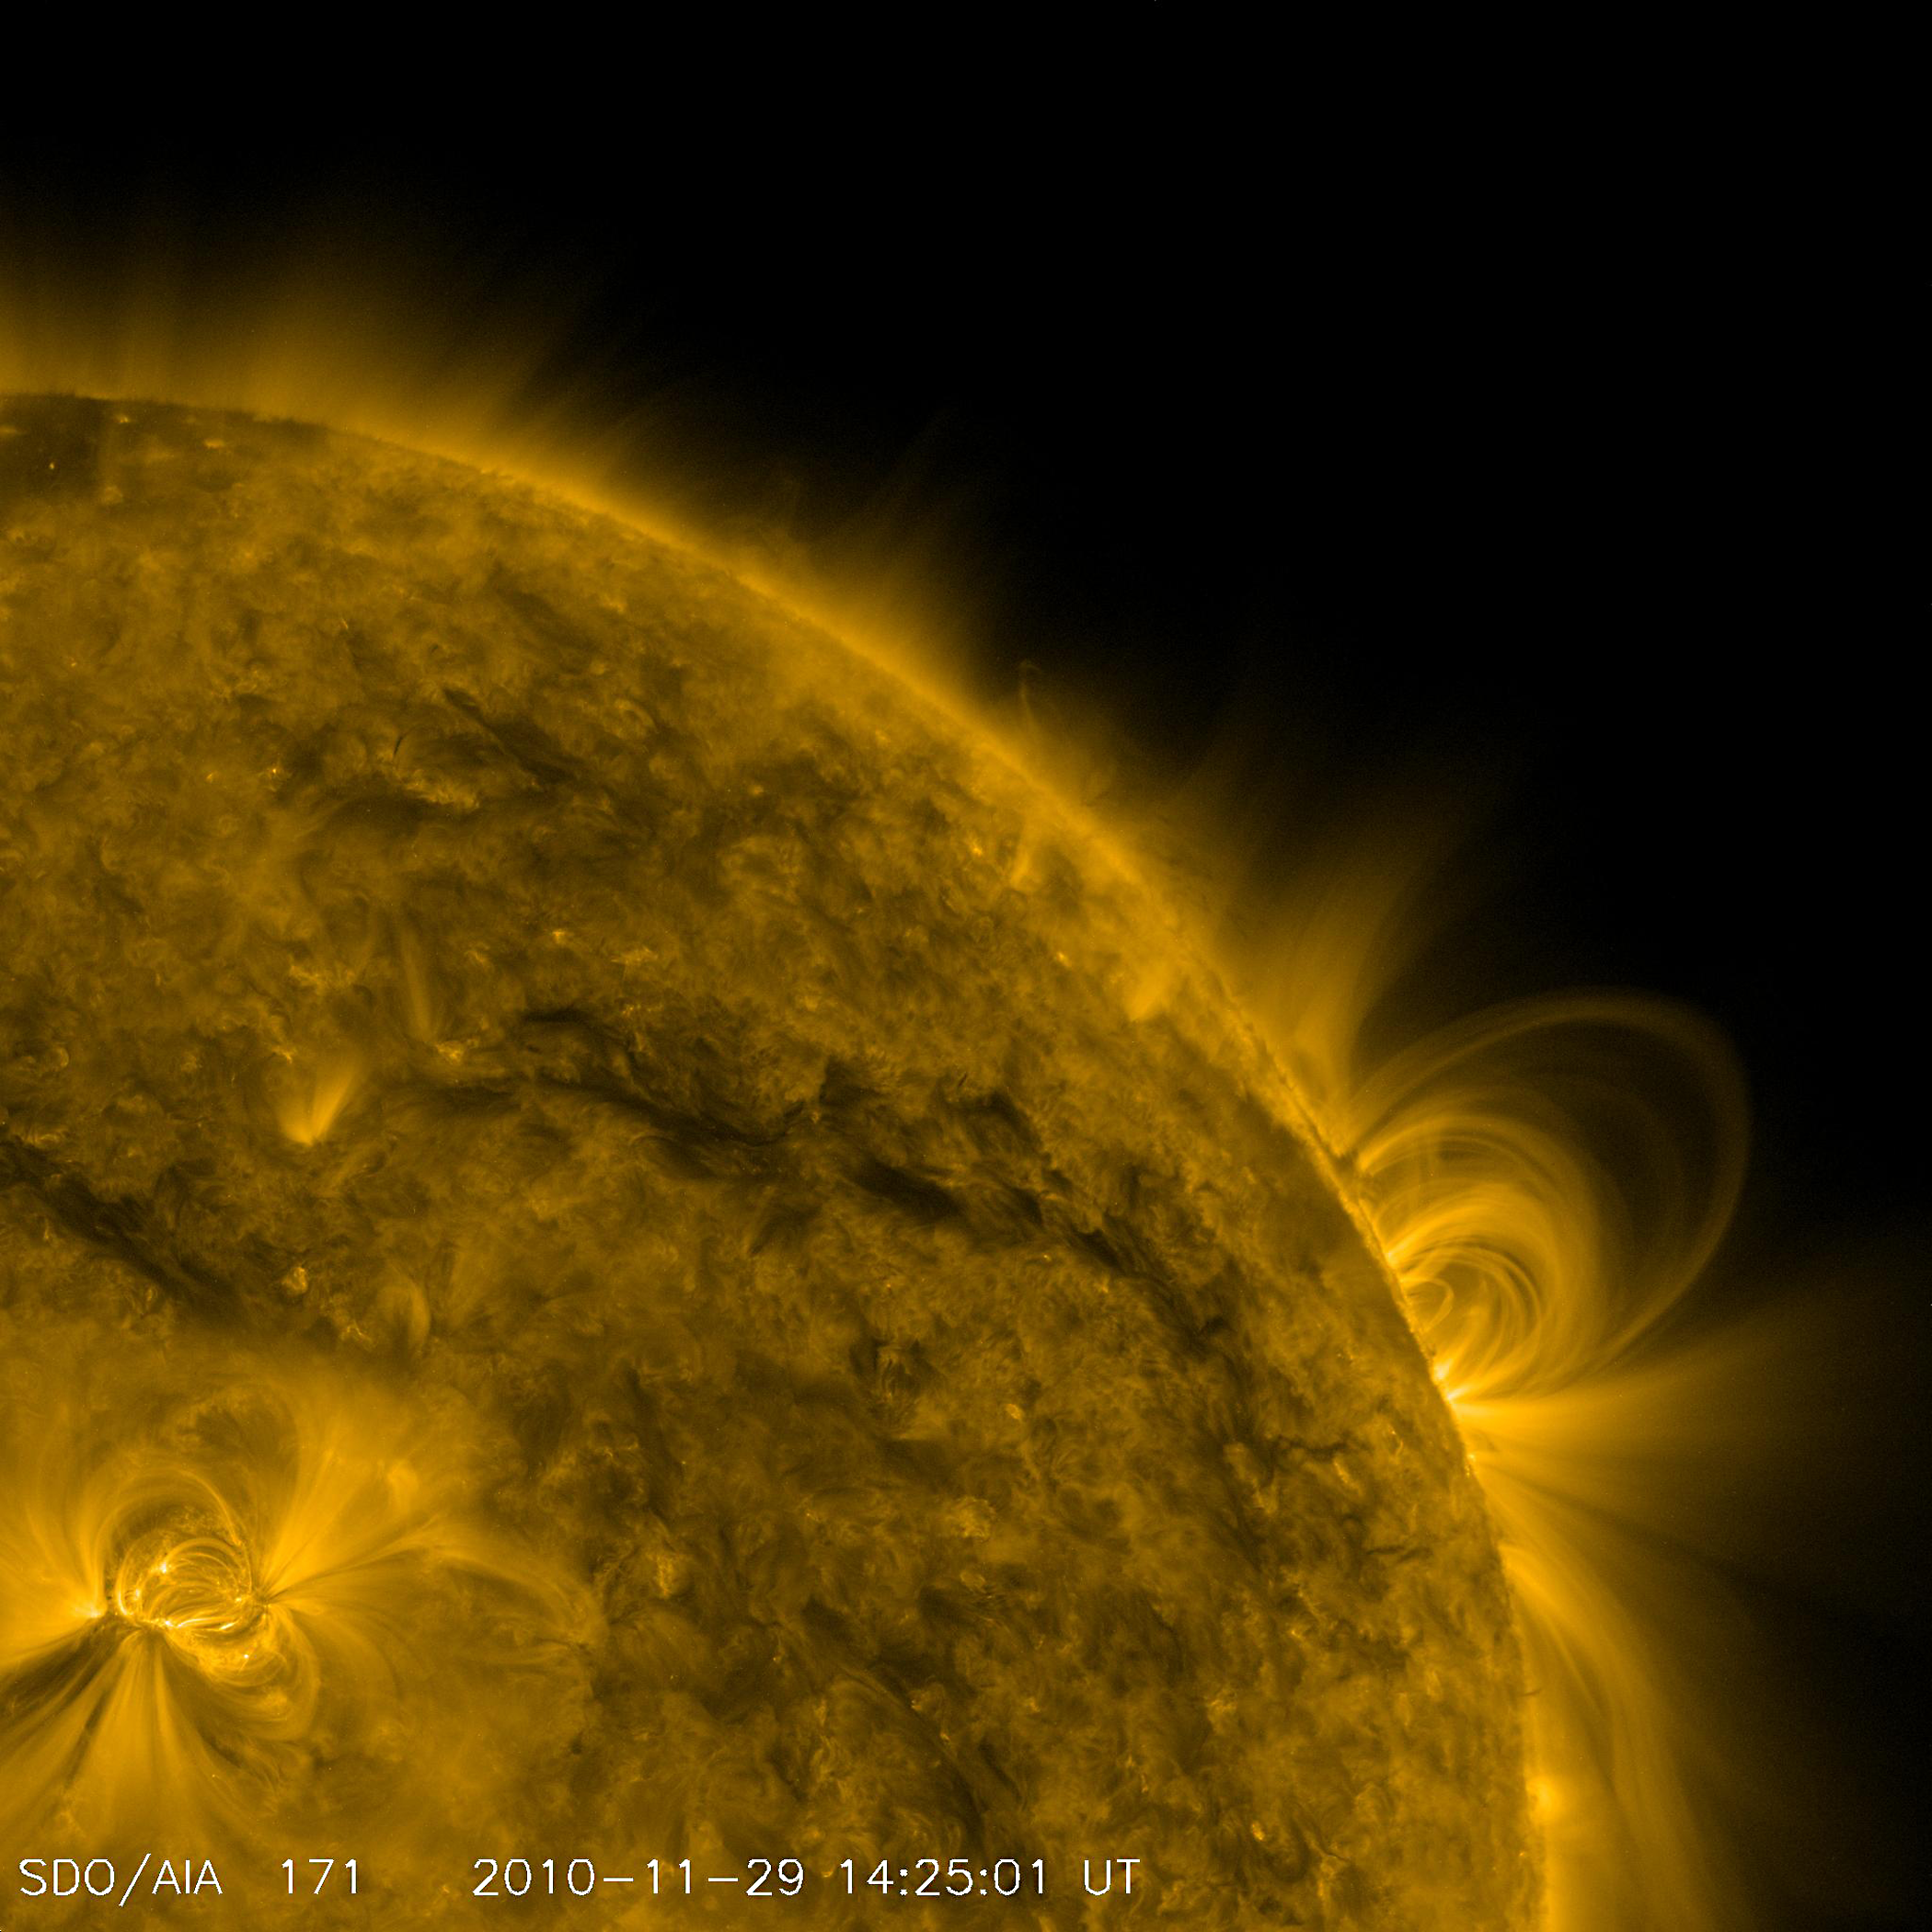
\includegraphics[width=0.6\textwidth]{figures/aia_171_loops_example.png}
	\caption{Image captured by the 171 \ang channel of the Atmospheric Imaging Assembly (AIA) onboard the Solar Dynamics Observatory (SDO). An arcade of loops in an active region can be seen on-disk in the lower left corner. Several prominent loop structures also appear off-limb on the right side. Image courtesy of NASA/SDO.}
	\label{fig:loops_example}
\end{figure}
%
\par Coronal loops, because of their relatively high temperatures ($\sim10^5-10^7$ K), are observed primarily in the extreme ultraviolet (EUV) and x-ray bands, with an associated wavelength range of $1\sim100$ \ang. While most coronal loop temperatures exceed $10^5$ K, loop plasma can span a range of temperatures and densities, due to both the complexity of the underlying field and the fact that individual loops are thermally isolated. As a result, loops are often categorized based on their thermal properties: \textit{cool}, 0.1-1 MK, \textit{warm}, 1-1.5 MK, and \textit{hot}, $\ge2$ MK \citep{reale_coronal_2010}. Whether these thermal categories actually represent distinct classes of loops or if they are all just transient states of the same type of loop is an open question in the coronal loops community, with the main debate revolving around whether different physical processes are at work in each type of loop. Additionally, loops have also been observed in several topologically different features on the Sun. See Table \ref{tab:loop_params} for some typical parameters associated with these distinct regions. This work will focus primarily on simulating loops in active regions, where many hot, nonflaring loops have been observed and emission from loop plasma is unlikely to be contaminated by radiation from the underlying transition region \citep{tripathi_emission_2011,warren_constraints_2011,warren_systematic_2012,winebarger_using_2011}. 
%\par Unfortunately, observational measurements of the coronal magnetic field are difficult and often involve a number of restrictive assumptions regarding the field topology and dynamics. Solar magnetograms can be constructed from measurements of the photospheric field through the effect of Zeeman splitting on spectral lines. The coronal field is then extrapolated, using the magnetogram as a lower boundary condition \citep[see][Ch. 5]{aschwanden_physics_2006}.
%
\begin{table}[htb]
	\centering
	\caption{Typical parameters for several different types of loops. Adapted from \citet{reale_coronal_2010}.\label{tab:loop_params}}
	\begin{tabular}{l | c c c}
		\hline\hline
		Region & $L$ [$10^9$ cm] & $T$ [$10^6$ K] & $n$ [$10^9$ cm$^{-3}$] \\
		\hline
		Bright points & 0.1-1 & 2 & 5 \\
		Active regions & 1-10 & 3 & 1-10 \\
		Giant arches & 10-100 & 1-2 & 0.1-1 \\
		Flaring loops & 1-10 & $>10$ & $>50$ \\
		\hline
	\end{tabular}
\end{table}
%
\section{Observations}
\label{sec:observations}
\hl{Discuss some observations of loops and what has been learned about them, what constraints, multi-stranded versus single stranded
Show some pretty pictures; if coronal loops are heated by nanoflares, what would be the observational signature?}
%
\par The first evidence of magnetically confined loop structures came from soft x-ray observations by grazing-incidence telescopes aboard rocket missions in the late 1960s as reported by \citet{vaiana_x-ray_1968}. Analysis of data from these early missions also allowed for classification of distinct topological features on the solar surface by \citet{vaiana_identification_1973} (see Table \ref{tab:loop_params}). These early findings provided the first look at the x-ray-bright, highly-structured corona; however, the short observing times of these rocket missions prevented systematic studies of these newly-discovered structures. The first sustained coronal loop observations did not come until the Orbiting Solar Observatory IV, equipped with a grazing-incidence x-ray telescope, and the x-ray telescope aboard the \textit{Skylab} space station \citep{krieger_results_1972,reale_coronal_2010}. Long observing times allowed for more accurate determinations of loop lifetimes, better comparisons between observations and loop models, and, perhaps most importantly, the finding that the coronal loop is the essential building block of all coronal structures \citep{rosner_dynamics_1978}. 
%
\par \hl{Need to introduce heating properties, frequency as the parameter we are most concerned about, review arguments for steady versus impulsive heating}
%
\par In order to make accurate determinations regarding the physical processes and properties of coronal loops, large statistical surveys are needed. However, isolating and analyzing individual loops is incredibly difficult, due primarily to inadequate instrument resolution relative to coronal length scales. In general, loop structures resolved by current observing instruments are considered to be \textit{multi-stranded}; that is, they are composed of many sub-resolution \textit{strands}, where a strand is the smallest loop for which the cross-section is isothermal \citep{bradshaw_diagnosing_2012}. 
%
\hl{Need something here about active region cores specifically and why we choose to study these over other parts of the AR}
%
\section{Modeling}
\label{sec:modeling}
%
\hl{Discuss modeling approaches, hydrodynamics versus magnetohydrodynamics, etc.}
\subsection{Static versus Dynamic}
\label{subsec:static_v_dynamic}
%
\hl{arguments for both; hydrostatic solutions briefly; scaling laws}
\hl{maybe combine MHD and hydrodynamics into single section, briefly mentioning MHD and why we discard the field}
\subsection{Magnetohydrodynamics}
\label{subsec:mhd}
%
\subsection{Hydrodynamics}
\label{subsec:hydro}
%
%
%?\subsection{Kinetic Modeling}
\section{Summary}
